\begin{figure*}[t!]
    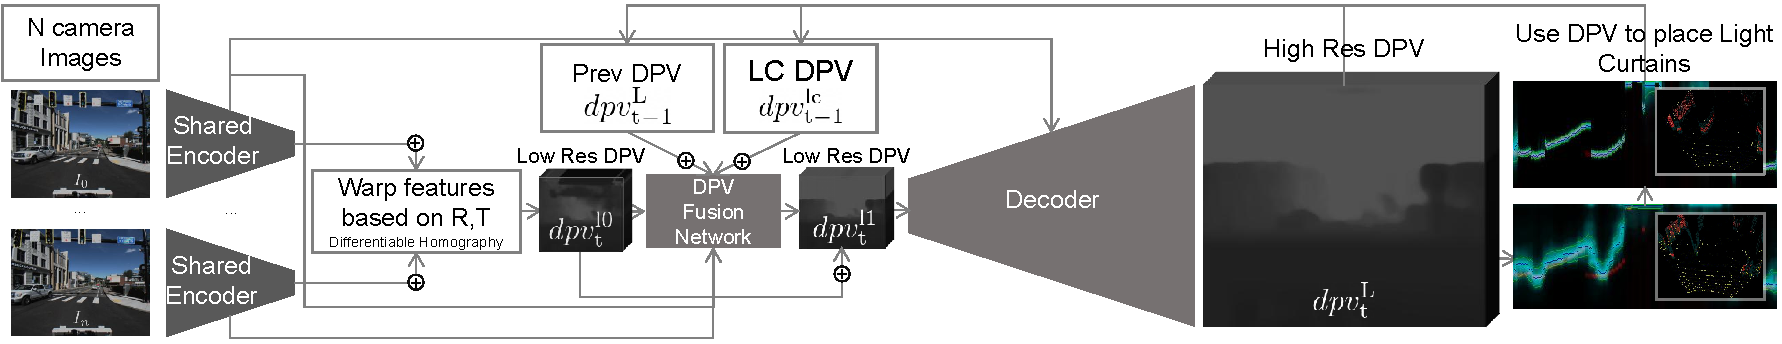
\includegraphics[width=1.0\textwidth]{figures/network.pdf}
    \caption{Our network takes in RGB images to generate a Depth Probability Volume, plans and places Light Curtains based on this DPV, and recursively refines it. This is then fed back on the next timestep to get much more refined DPV estimate. }
    \label{fig:network}
\end{figure*}
    
\section{Network Architecture}

\subsection{Motivation}

While starting from a uniform or gaussian prior with a large uncertainity is a valid option, it is slow to converge. Furthermore, a Light Curtain only means of depth estimation is extracted primarily along the ruled placement of the curtain, at least based on our above placement policies. We would ideally like to use information from a Monocular RGB camera or Stereo Pair to initialize our prior, with a similar DPV representation. To this end, a Deep Learning based architecture is ideal, and we also reason that such an architecture could potentially learn to fuse/incorporate information from both modalities better.

\subsection{Structure of Network}

The first step is to build a network that can generate DPV's similar to our light curtain only estimation strategy from RGB images. To this end, we build upon the MVSNet/PSMNet architecture. N images, usually 2 $I_{0}, I_{1}$ are fed into encoders that share weights, and the features are then warped into different fronto-parallel planes of the reference image $I_{0}$ using pre-computed $R_{i}^{0}, t_{i}^{0}$. Further convolutions are run to generate a low resolution DPV $dpv_{\mathrm{t}}^{\mathrm{l0}}$ [80, 96] where the log softmax operator is applied and regressed on. The transform between the camera's act as a constraint, forcing the feature maps learnt to respect depth to channel correspondence. The add operator into a common feature map is analagous to adding probabilities in log-space. 

This is then fed into the DPV Fusion Network (Set of 3D Convolutions) that incorporate a downsampled version of $dpv_{\mathrm{t-1}}^{\mathrm{L}}$ along with the the light curtain DPV that we had applied recursive bayesian updates on $dpv_{\mathrm{t-1}}^{\mathrm{lc}}$, and a residual is computed and added back to $dpv_{\mathrm{t}}^{\mathrm{l0}}$ to generate $dpv_{\mathrm{t}}^{\mathrm{l1}}$ to be regressed upon similarly. Occasionally, we train without this feedback by inputting a uniform distribution. Finally, this is then passed into a decoder with skip connections to generate a high resolution DPV $dpv_{\mathrm{t}}^{\mathrm{L}}$. This is then used to plan and place light curtains, from which we generate a new $dpv_{\mathrm{t}}^{\mathrm{lc}}$ to be fed in the next stage.

\subsection{Loss Functions}

\textbf{Soft Cross Entropy Loss:} We build upon the ideas found in \cite{Yang-2019-118007} and use a soft cross entropy loss function, with the ground truth lidar depthmap becoming a gaussian DPV with $\sigma_{gt}$ instead of a one hot vector. This way, when taking $\mathbb{E}\left(dpv^{gt}\right)$ we get the exact depth value instead of an approxmiation limited by the depth quantization $D_{c}$. We also make the quantization slightly non-linear to have more steps between objects that are closer to the camera.

\small
\begin{align}
    l_{sce}=\frac{-\sum_{i}\sum_{d}\left(dpv^{\mathrm{\{l0,l1,L\}}}*log\left(dpv^{gt}\right)\right)}{n} \\
    D_{c}=\left\{ d_{0},...d_{n}\right\} \quad d_{i}=d_{min}+(d_{max}-d_{min})*t^{pow}
   \label{eq:seloss}
\end{align}
\normalsize

\textbf{L/R Consistency Loss:} We train on both the Left and Right Images of the stereo pair where the Projection matrices $P_{l}, P_{r}$ are known. We enforce predicted Depth and RGB consistency by warping the Left Depthmap/Projected RGB into the Right Camera and vice-versa, and minimize the following metric:

\small
\begin{align}
    D_{l}=\mathbb{E}\left(dpv_{l}^{L}\right)\qquad D_{r}=\mathbb{E}\left(dpv_{r}^{L}\right) \\
    l_{dcl}=\frac{1}{n}\sum_{i}\left(\frac{\left|D_{\{l,r\}}-w\left(D_{\{r,l\}},P_{\{l,r\}}\right)\right|}{D_{\{l,r\}}+w\left(D_{\{r,l\}},P_{\{l,r\}}\right)}\right) \\
    l_{rcl}=\frac{1}{n}\sum_{i}\left(||I_{\{l,r\}}-w\left(I_{\{r,l\}},D_{\{l,r\}},P_{\{l,r\}}\right)||_{1}\right)
   \label{eq:lrcons} 
\end{align}
\normalsize

\textbf{Edge aware Smoothness Loss:} We ensure that neighbouring pixels have consistent surface normals, except on the edges/boundaries of objects with the Sobel operator $S_{x}, S_{y}$ via the term:

\small
\begin{align}
    l_{s}=\frac{1}{n}\sum_{i}\left(\left|\frac{\partial I}{\partial x}\right|e^{-|S_{x}I|}+\left|\frac{\partial I}{\partial y}\right|e^{-|S_{y}I|}\right)
   \label{eq:smooth} 
\end{align}
\normalsize

\subsection{Datasets}

We train and validate our algorithms on the KITTI dataset. We then trained the same network by initializing on those weights, but using our custom ILIM dataset to evaluate our algorithms on our sensor platform / jeep.

\section{RGB + Light Curtain Experiments}

\textbf{Effects of our loss function:} We do some simple experiments, training the task of monocular depth estimation, and we explore the effects of enabling/disabling the various loss functions:

\noindent
\begin{table}[h]
   \centering
   \resizebox{0.7\linewidth}{!}{
   \begin{tabular}{|l|l|}
   \hline
    Parameters&  RMSE/m\\ \hline
    $\sigma_{gt}=0.05$ &3.24  \\ \hline
    $\sigma_{gt}=0.2$ &3.16  \\ \hline
    $\sigma_{gt}=0.3$ &3.06  \\ \hline
    $\sigma_{gt}=0.3$ with $l_{dcl}, l_{rcl}$  &2.93  \\ \hline
    $\sigma_{gt}=0.3$ with $l_{dcl}, l_{rcl}, l_{s}$  &2.90  \\ \hline
   \end{tabular}}
   \caption{Effects of various loss functions for the baseline of Monocular Depth Estimation only}
   \label{table:xx}
\end{table}

We note succesively improving performance as we increase $\sigma_{gt}$, with poorer performance when the depth is effectively encoded as a one-hot vector (eg. $\sigma_{gt}=0.05$), since the depth was more likely to be forced into one of the categories in $D_{c}$. Adding in $l_{dcl}, l_{rcl}$ and $l_{s}$ improved performance further, but we did not see any significant performance improvement in varying $t^{pow}$ especially once $\sigma_{gt}$ was increased.

\textbf{Effect of Stereo Inputs:} We experiment with passing in a Monocular Pair at $t, t-1$, or a Stereo Pair at $t$, with $R,t$ known in both cases. We note significantly better performance with Stereo input. Note that our method can generalize to any N camera setup. Results seen in ~\ref{fig:stereodpv}

\textbf{Effect of DPV Fusion Network:} We consider the task of Lidar Upsampling. The Velodyne Lidar in the KITTI dataset, can be converted into a low resolution depthmap, and consequently a low res DPV we call $dpv_{t}^{gt}$ . We could then fuse both $dpv_{t}^{l0}$ and $dpv_{t}^{gt}$ to generate $dpv_{t}^{l1}$ using Bayesian Inference. Alternatively, we could feed both of those inputs into our DPV Fusion Network above. We note improved performance in this upsampling task when using this approach as seen in ~\ref{fig:stereodpv}. 

\begin{figure}[h]
   \centering
   \begin{minipage}{0.5\textwidth}
       \centering
       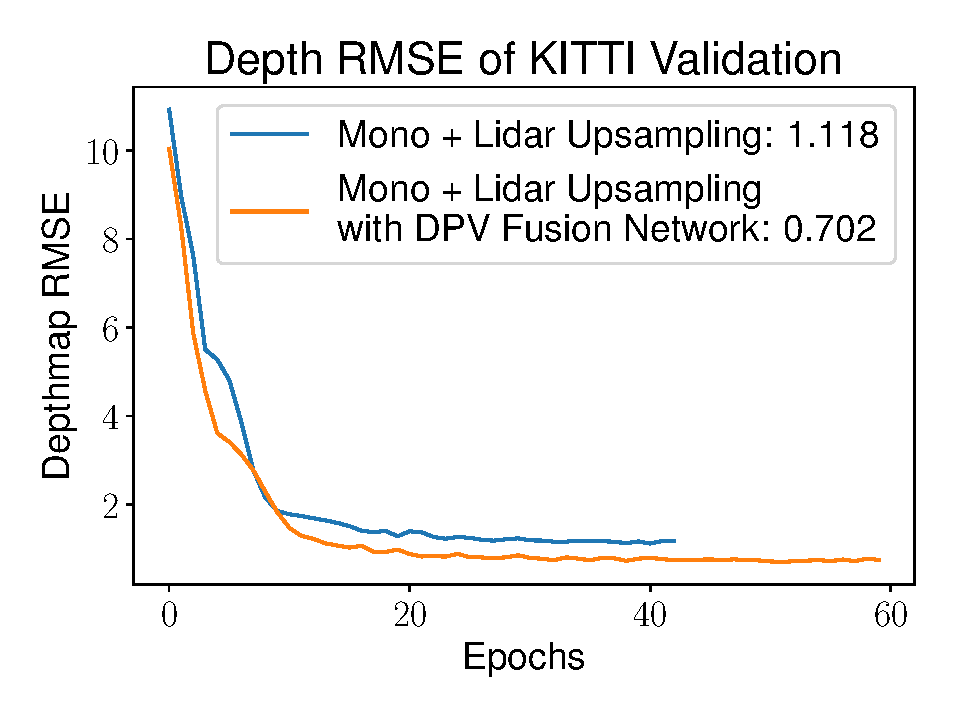
\includegraphics[width=0.49\textwidth]{figures/Figure_6.pdf}
       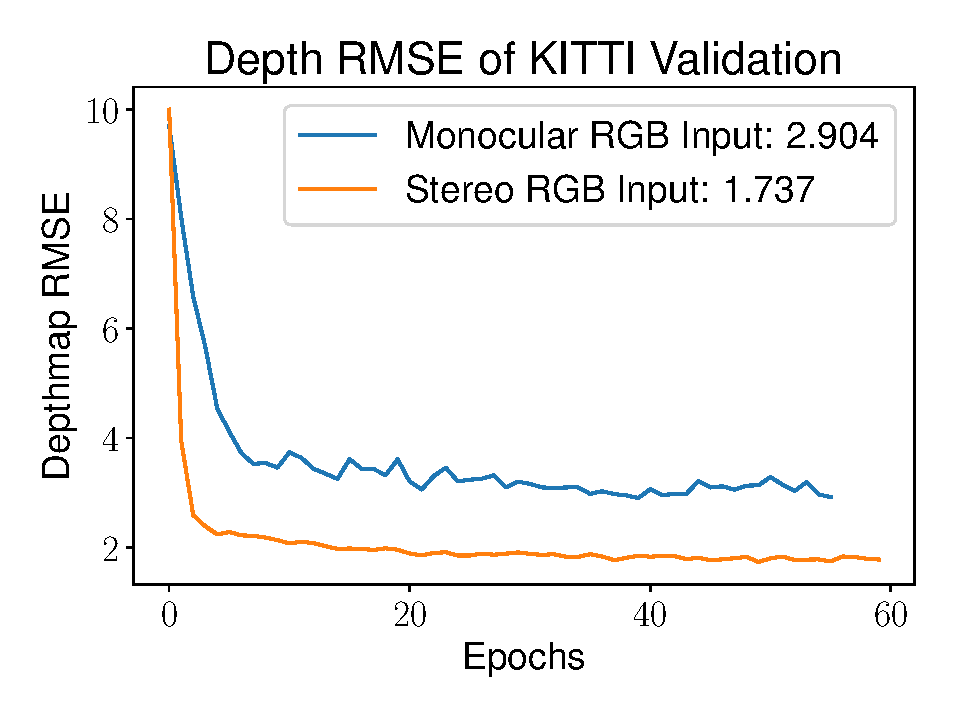
\includegraphics[width=0.49\textwidth]{figures/Figure_7.pdf}
   \end{minipage}\hfill
   \centering
   \caption{ \textbf{Left:} Same network but having a Stereo Pair at $t$ passed in instead of Monocular Pair at $t, t-1$. \textbf{Right:} Fusing the GT Lidar data with $dpv_{t}^{l0}$ to generate $dpv_{t}^{l1}$ and $dpv_{t}^{L}$ with Bayesian Inference vs DPV Fusion Network}
   \label{fig:stereodpv} 
\end{figure}

\textbf{Effect of a Stronger Prior:} Here, we show that a prior generated from a monocular RGB camera yields higher accuracy and faster convergence. Results seen in ~\ref{fig:prior} 

\begin{figure}[h]
   \centering
   \begin{minipage}{0.5\textwidth}
       \centering
       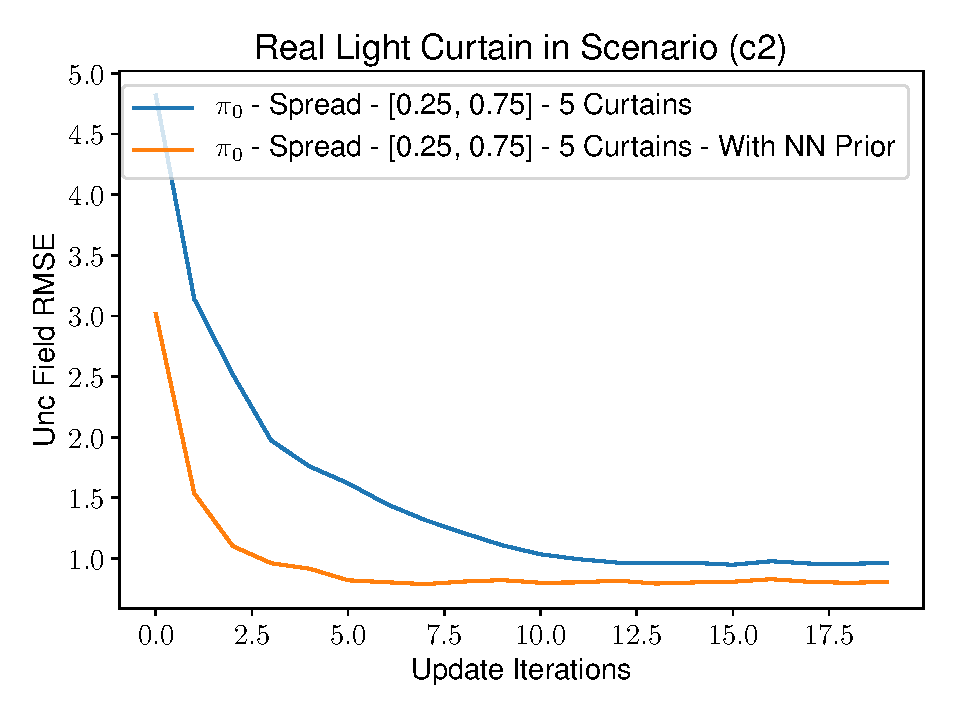
\includegraphics[width=0.49\textwidth]{figures/figure_X.pdf}
       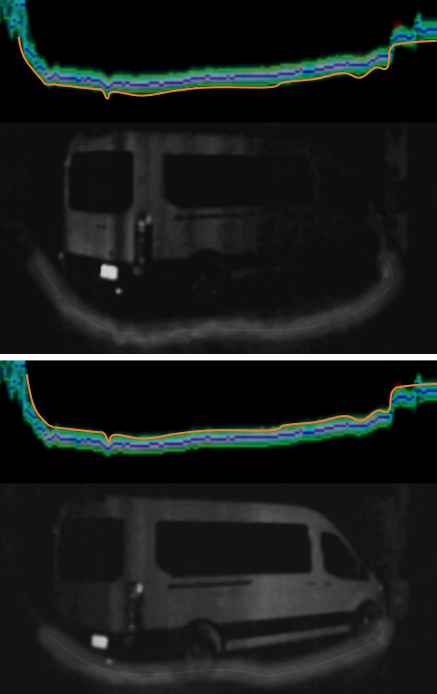
\includegraphics[width=0.29\textwidth]{figures/placement3.png}
   \end{minipage}\hfill
   \centering
   \caption{ \textbf{Right:} Starting from a Prior distribution from a Monocular Depth Network leads to faster convergence. \textbf{Left:} Policy $m0$ placing curtains along 3 Locations of a prior distribution from a Monocular Depth Network as seen in the Light Curtain's NIR image.}
   \label{fig:prior} 
\end{figure}

\textbf{Effect of a Stronger Prior:} Here, we show that a prior generated from a monocular RGB camera yields higher accuracy and faster convergence. Results seen in ~\ref{fig:prior} 


\iffalse
Generating Prior from RGB
   NN Formulation figure
   Soft CE, QPower, Left/Right Consistency (RGB + Depth), Smoothness
   Experiments:
      Show table for above
   LC Integration
   Experiments:
      Effect/Speedup of having a Prior
      
      3D Upsampling of Lidar
      Time feedback vs no
      Deep Learning vs no Deep Learning (Ruled Surface etc.)

      experiment does actually seeing uncertinayt make a difference

      move experiment prior to other part
      
      experiment for deep learning based full depth vs unc depth of no deep learning

      Outdoor Experiments:
   etc.
Future Work
\fi






